\section{Проект}
\subsection{Средства реализации}
\noindent\indent При разработке использовался язык программирования C/C++,
как основной язык разработки системы моделирования <<Sputnix Satellite Modeller>>.
Так же использовались следующие продукты:
\begin{itemize}
    \item OpenGL, freeglut, glu -- для визуализации данных
    \item Google Test -- для юнит-тестирования компонентов
\end{itemize}
\subsection{Модули и алгоритмы}
\noindent\indent Интерфейс системы делится на две основные части: визуализирующую и
модельную.\par
    К модельной относятся:
\begin{itemize}
    \item \code{helper::container} -- пространство имен, содержащее два контейнера:
    \code{SailParameters} (содержит значения атрибутов паруса) и
    \code{KeplerParameters} (содержит кеплеровы элементы орбиты);
    \item \code{helper::shadow} -- пространство имен, содержащее интерфейс <<функции тени>>,
    и её вспомогательных функции;
    \item \code{helper::orbit} -- пространство имен, содержащее интерфейсы вспомогательных
    функций для расчета различных элементов орбиты;
    \item \code{helper::optimization} -- пространство имен, содержащее методы оптимизации
    решения;
    \item \code{helper::integral} -- пространство имен, содержащее методы интегрирования
    функций;
    \item \code{helper::constant} -- пространство имен, содержащее различные физические
    константы;
    \item \code{force} -- пространство имен функций расчета возмущающих сил;
    \item \code{kepler::Differentials} -- класс по рассчету значений изменения кеплеровых
    элементов орбиты;
    \item \code{math::object} -- класс, созданный для хранения и изменения
    позиции, ориентации и размерности объекта;
    \item \code{phys::object} -- наследник класса \code{math::object}, содержащий дополнительные
    параметры массы, скорости и угловой скорости;
    \item \code{math::model::SatelliteOrbit} -- главный класс, предназначенный для
    моделирования внешних воздействий и подбора оптимальных угловых значений.
\end{itemize}
    К визуализирующей относятся:
\begin{itemize}
    \item \code{glsl::shader} -- пространство имен, содержащее класс шейдера \code{shader} и
    шейдерной программы \code{program}, а также класс исключения \code{error};
    \item \code{helper::color} -- класс для хранения значений цвета;
    \item \code{draw::object} -- интерфейс объекта хранения модели и цвета;
    \item \code{glsl::object} -- интерфейс для привязки индексов объектов шейдерной
    программы;
    \item \code{shape::solid::sphere} -- класс отрисовки сфер;
    \item \code{shape::line} -- класс отрисовки линий;
\end{itemize}
\subsubsection{Интерфейс \code{helper::container::SailParameters}}
\noindent\indent Поля:
\begin{itemize}
    \item \code{Bf}, \code{Bb} -- коэффициенты, показывающие характер индикатрисы отражения
    за вычетом зеркальной составляющей;
    \item \code{ef}, \code{eb} -- излучательная способность освещенной и обратной стороны паруса
    \item \code{rho} -- коэффициент зеркального отражения;
    \item \code{s} -- коэффициент зеркальности;
    \item \code{area} -- площадь элементарной части паруса
    \item \code{norm} -- нормаль, восстановленная от поверхности элементарной части паруса.
\end{itemize}
\subsubsection{Интерфейс \code{helper::container::KeplerParameters}}
\noindent\indent Поля:
\begin{itemize}
    \item \code{e} -- эксцентриситет орбиты;
    \item \code{p} -- параметр орбиты;
    \item \code{omega} -- аргумент перигея;
    \item \code{i} -- наклонение;
    \item \code{Omega} -- долгота восходящего узла;
    \item \code{tau} -- параметр положения объекта на орбите в каждый момент времени.
\end{itemize}
\subsubsection{Интерфейс \code{helper::shadow}}
\noindent\indent Функции:
\begin{itemize}
    \item \code{shadowFunction(Vector r, Vector rSE)} -- вычисляет значение
    функции тени в диапазоне [0, 1], при заданных значениях радиус-вектора, направленного
    из центра Земли к центру масс аппарата (\code{r}) и вектору, направленному из центра Солнца
    к центру Земли (\code{rSE});
    \item \code{angle(Vector r, Vector rSE)} -- функция расчета угла между радиус вектором спутника
    и вектором, направленным из центра Солнца к центру Земли (\code{rSE});
    \item \code{shadow2Angle(Vector r, Vector rSE)} -- функция расчета максимального
    угла перехода между областью полутени и области без тени;
    \item \code{shadowAngle(Vector r, Vector rSE)} -- функция расчета максимального
    угла перехода между областями полутени и тени;
    \item \code{shadowAngleThrowOmega(Vector r, Vector rSE, double tgOmega)} --
    функция расчета угла тени/полутени, в зависимости от переданного параметра
    тангенса угла наклона (\code{tgOmega});
\end{itemize}
\subsubsection{Интерфейс \code{helper::orbit}}
\noindent\indent Функции:
\begin{itemize}
    \item \code{E(helper::container::KeplerParameters kepParams,
                  double mainMass,
                  double satMass,
                  double t,
                  double epsilon)} -- функция расчета эксцентрической аномалии;
    \item \code{nu(helper::container::KeplerParameters kepParams, double E)} --
    функция расчета истинной аномалии;
    \item \code{r(helper::container::KeplerParameters kepParams, double E)} --
    функция расчета длины радиус-вектора, соединяющего фокус с точкой орбиты;
    \item \code{r(double r, double nu)} -- функция вычисления значения радиус-вектора
    в плоскости орбиты;
    \item \code{r(helper::container::KeplerParameters kepParams, Vector r)} --
    функция расчета значения радиус-вектора в орбитальную систему координат;
    \item \code{T(helper::container::KeplerParameters kepParams, double mainMass, double satMass)} --
    функция расчета периода обращения вокруг заданной орбиты.
\end{itemize}
\subsubsection{Интерфейс \code{helper::optimization}}
\noindent\indent Функции:
\begin{itemize}
    \item \code{gradient(Function fun, bool maximization, size\_t countArgs,
    Vector minVals, Vector maxVals, double delta, double epsilon, size\_t MAX\_ITERATIONS)} --
    функция поиска оптимальных параметров заданной функции градиентным методом;
    \item \code{full(Function fun, bool maximization, size\_t countArgs,
    Vector minVals, Vector maxVals, delta)} -- функция поиска оптимальных параметров
    заданной функции методом <<грубой силы>>;
    \item \code{genetic(Function function, bool maximization, size\_t countArgs,
    Vector minVals, Vector maxVals, double delta, size\_t MAX\_ITERATIONS,
    size\_t initialPopulation, size\_t populationSize, size\_t countCrossovers,
    size\_t countMutations, double scaleFactor)} -- функция поиска оптимальных
    параметров заданной функции с помощью генетического алгоритма;
    \item \code{amoeba(Function function, bool maximization, size\_t countArgs,
    Vector minVals, Vector maxVals, size\_t MAX\_ITERATIONS)} -- функция поиска
    оптимальных параметров заданной функции с помощью адаптивного алгоритма Нелдера-Мида.
\end{itemize}
\subsubsection{Интерфейс \code{helper::integral}}
\noindent\indent Функции:
\begin{itemize}
    \item \code{rect(function f, double from, double to, double dh)} -- функция
    поиска значения интеграла функции на заданном интервале методом прямоугольников;
    \item \code{trapez(function f, double from, double to, double dh)} -- функция
    поиска значения интеграла функции на заданном интервале методом трапеций;
    \item \code{simpson(function f, double from, double to, double dh)} -- функция
    поиска значения интеграла функции на заданном интервале методом Симпсона;
\end{itemize}
\subsubsection{Интерфейс \code{helper::constant}}
\noindent\indent Константы:
\begin{itemize}
    \item \code{G} -- гравитационная постоянная;
    \item \code{EARTH\_R} -- радиус Земли;
    \item \code{EARTH\_E\_R} -- экваториальный радиус Земли;
    \item \code{EARTH\_P\_R} -- полярный радиус Земли;
    \item \code{EARTH\_MASS} -- масса Земли;
    \item \code{ATMOSPHERIC\_PRESSURE\_0} -- нормальное атмосферное давление;
    \item \code{TEMPERATURE\_0} -- нормальная температура;
    \item \code{J2} -- вторая зональная гармоника;
    \item \code{C\_d} -- коэффициент лобового атмосферного сопротивления;
    \item \code{EARTH\_OMEGA} -- скорость вращения Земли вокруг своей оси;
    \item \code{SOLAR\_PRESSURE} -- значение солнечного давления света вблизи Земли;
    \item \code{SUN\_RADIUS} -- радиус Солнца;
    \item \code{SUN\_MASS} -- масса Солнца;
    \item \code{EARTH\_ECCENTRICITY} -- эксцентриситет орбиты Земли;
    \item \code{EARTH\_SEMIMAJOR\_AXIS} -- величина большей полуоси орбиты Земли;
    \item \code{EARTH\_INCILATION} -- наклонение орбиты Земли;
    \item \code{EARTH\_LONGITUDE\_ASCENDING\_NODE} -- долгота восходящего узла орбиты Земли;
    \item \code{EARTH\_ARGUMENT\_PERAPSIS} -- аргумент перигея орбиты Земли;
    \item \code{EARTH\_ECLIPTIC} -- угол наклонения эклиптики Земли.
\end{itemize}
\subsubsection{Интерфейс \code{force}}
\noindent\indent Функции:
\begin{itemize}
    \item \code{gravJ2(
    helper::container::KeplerParameters params,
    double mass,
    double mu,}


    \code{double r,
    double nu
    )} -- функция рассчета силы, учитывающей действие второй зональной гармоники;
    \item \code{atmos(
    helper::container::KeplerParameters params,
    double rho\_atm,}
    \code{double sail\_area,
    Vector sail\_norm,
    double mu, double r, double nu
    )} -- функция расчета силы сопротивления воздуха;
    \item \code{solar(
    helper::container::SailParameters params,
    Vector solar\_norm
    )} -- функция расчета силы, возникающей под действием солнечного давления.
\end{itemize}
\subsubsection{Интерфейс \code{kepler::Differetials}}
\noindent\indent Методы:
\begin{itemize}
    \item \code{operator()(
    helper::container::KeplerParameters params,
    phys::object main,}


    \code{phys::object sat,
    double t,
    Vector force
    )} -- метод (функтор) расчета значений изменения кеплеровых элементов орбиты.
    Возвращает вектор значений ($[
        \frac{dp}{dt},\,\,
        \frac{de}{dt}\,\,
        \frac{d\omega}{dt}\,\,
        \frac{di}{dt}\,\,
        \frac{d\Omega}{dt}\,\,
        \frac{d\tau^*}{dt}
    ]$)
    \item \code{dexdt(double r,
        double mu,
        double nu,
        helper::container::KeplerParameters params,
        Vector f
    )} -- метод расчета изменения <<наклоненного>> эксцентриситета на $\cos(\omega)$;
    \item \code{deydt(double r,
        double mu,
        double nu,
        helper::container::KeplerParameters params,
        Vector f
    )} -- метод расчета изменения <<наклоненного>> эксцентриситета на $\sin(\omega)$;
    \item \code{dudt(double r,
        double mu,
        double nu,
        helper::container::KeplerParameters params,
        Vector f
    )} -- метод расчета изменения широты орбиты;
\end{itemize}
\subsubsection{Класс \code{math::object}}
\noindent\indent Поля:
\begin{itemize}
    \item \code{m\_position} -- вектор позиции объекта;
    \item \code{m\_scale} -- вектор масштабировани объекта;
    \item \code{m\_orientation} -- матрица ориентации объекта.
\end{itemize}\par
    Методы:
\begin{itemize}
    \item \code{rotate(Vector axis, double angle)} -- метод вращения объекта
    вокруг заданной оси;
    \item \code{orientation(Matrix orientation)} -- метод задания новой матрицы
    ориентации;
    \item \code{scale(Vector src)} -- метод задание масштабирования объекта;
    \item \code{move(Vector dv)} -- метод перемещения объекта;
    \item \code{position()} -- метод получения текущего положения объекта;
    \item \code{scale()} -- метод получения текущей матрицы масштабирования;
    \item \code{orientation()} -- метод получения текущей матрицы ориентации объекта.
\end{itemize}
\subsubsection{Класс \code{phys::object}}
\noindent\indent Поля:
\begin{itemize}
    \item \code{m\_dw} -- вектор угловой скорости;
    \item \code{m\_dv} -- вектор скорости;
    \item \code{m\_mass} -- масса объекта.
\end{itemize}\par
    Методы:
\begin{itemize}
    \item \code{update\_dw(Vector src)} -- метод изменения угловой скорости;
    \item \code{update\_dv(Vector src)} -- метод изменения скорости;
    \item \code{update(double dt)} -- метод <<обновления>> текущих параметров позиции
    и ориентации согласно собственной угловой скорости и скорости движения;
    \item \code{dw()} -- метод получения текущей угловой скорости;
    \item \code{dv()} -- метод получения текущей скорости;
    \item \code{mass()} -- метод получения значения массы объекта.
\end{itemize}
\subsection{Анализ физической модели}
\noindent\indent Т.к. в данной конкретной задаче необходимо увеличить высоту орбиты
спутника на максимальную высоту в заданный промежуток времени, а наибольший эффект
на это оказывают две компоненты: параметр орбиты и эксцентриситет орбиты, то естественно
сделать акцент на максимизации данных параметров.\par
    Как видно из системы (\ref{fig:ForcesOrientation}), - на прирост данных параметров
влияют силы, направленные вдоль радиального вектора и вдоль в вектора скорости.\par
    Рассмотрим зависимость суммы первых двух компонент возмущающих сил и углов ориентации аппарата:
\begin{figure}[h]
  \centering
  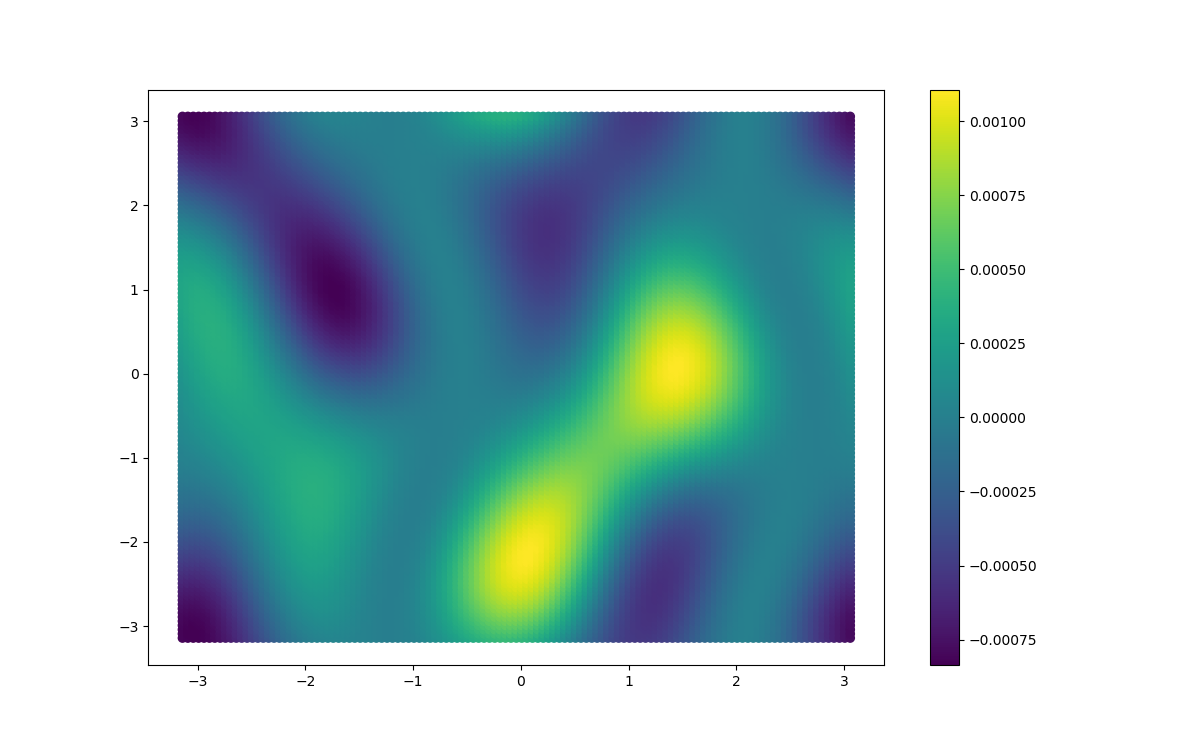
\includegraphics[width=0.8\textwidth]{experiments/FirstExperiment}
  \caption{Зависимость силы солнечного давления от углов}
  \label{fig:Force2Angles}
\end{figure}\par
    Как видно из графика, функция имеет несколько локальных максимумов, причем,
между двумя наибольшими экстремумами расположено нечто подобное седлу. Также
рассмотрим график функции зависимости значений дифференциалов эксцентриситета и
параметра орбиты:
\begin{figure}[h]
  \centering
  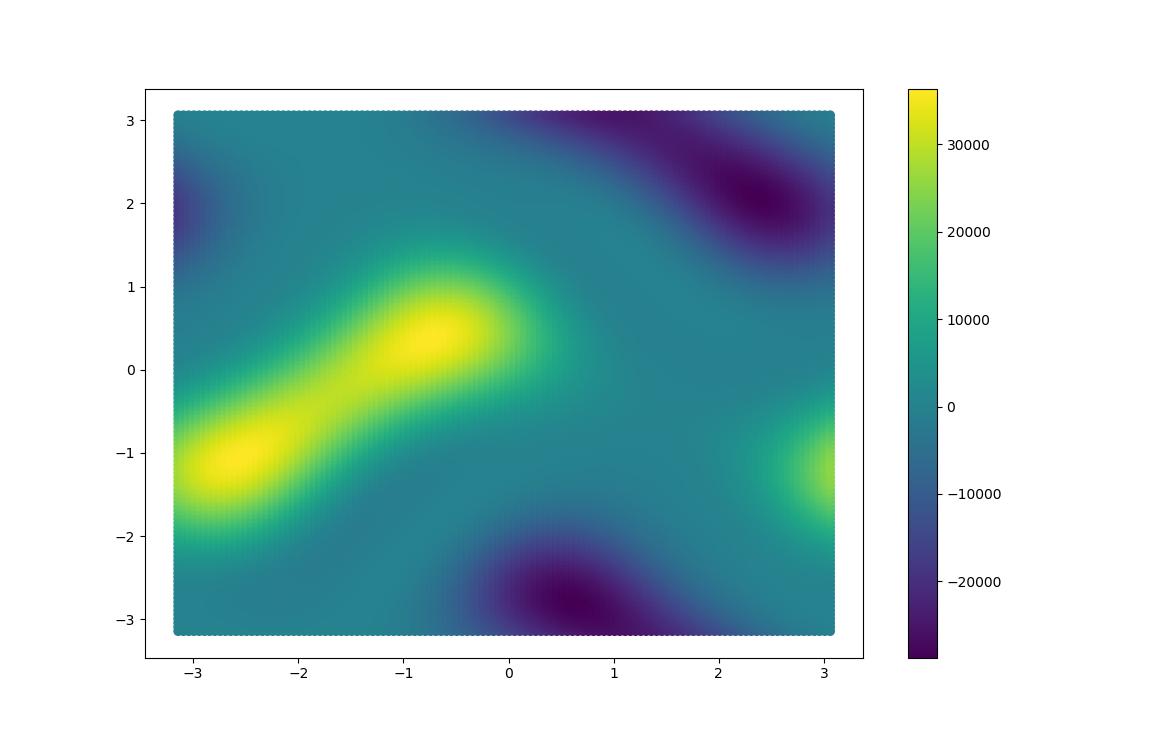
\includegraphics[width=0.8\textwidth]{experiments/SecondExperiment}
  \caption{Зависимость изменения параметров орбиты от ориентации спутника}
  \label{fig:KeplerParams2Angles}
\end{figure}\par
    Также, как и в предыдущем графике, существует седловина между двумя наибольшими
экстремумами функции, и при этом, существует как минимум ещё один локальный максимум.
    Из чего можно сделать предположение, что градиентный метод в условиях данной
задачи не будет достаточным для поиска глобального максимума функции.
